\setlength{\footskip}{8mm}

\chapter{Experimental Results}
\label{ch:results}

\textit{The test rover was manually controlled in two conditions, indoor and outdoor. The video feed and the IMU data was collected and then ORB and VIORB SLAM were executed on them. The results of the two experiments are discussed in this section. }


\section{Experiment Enviroment}

The test rover as shown in figure \ref{fig:rigsetup} (c), was manually controlled and a laptop was connected to the camera and flight controller. The data collected by the laptop was stored in a ROS bag file. The bag file was replayed and the collected data was used to run VIORB and ORB SLAM. 

\section{Indoor Experiment}
\begin{figure} [!h]
	\centering
	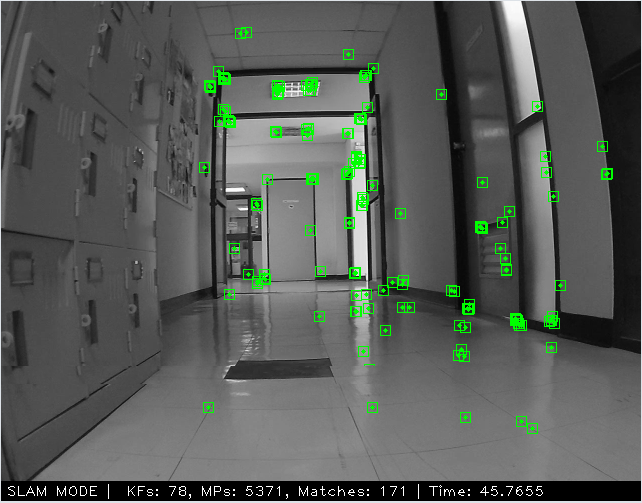
\includegraphics[width=5in]{figures/demo2_screen}
	\caption[Indoor experiment environment]{\small 
		Indoor experiment environment. }
	\label{fig:indoor-experiment-live}
\end{figure}

The test rover was run in an indoor environment for 170 seconds, as shown in Figure~\ref{fig:indoor-experiment-live}. The number of ORB features to extract was kept as 2000. The approximate length of the path was 17 meters. The keypoints, trajectory, and pointclouds generated by both algorithms are shown in Figure~\ref{fig:indoor-path-visualization}.

The test rover while moving on the ground produced a lot of jerky movements and it affected VIORB SLAM more than ORB SLAM. VIORB SLAM re-localized a couple of times. It could be re-localize after 117.459 seconds. Tracking was lost when the rover was making a left turn and the number of features was relatively low compared to other frames.

ORB SLAM tracked the environment for the entire duration of the test. There were errors in tracking because the rover returned halfway between the path it took. This was because the hallway was darker on its return path and features could not be detected precisely. 


\begin{figure}[h]
	
	\centering1
	\subfloat[]{%
		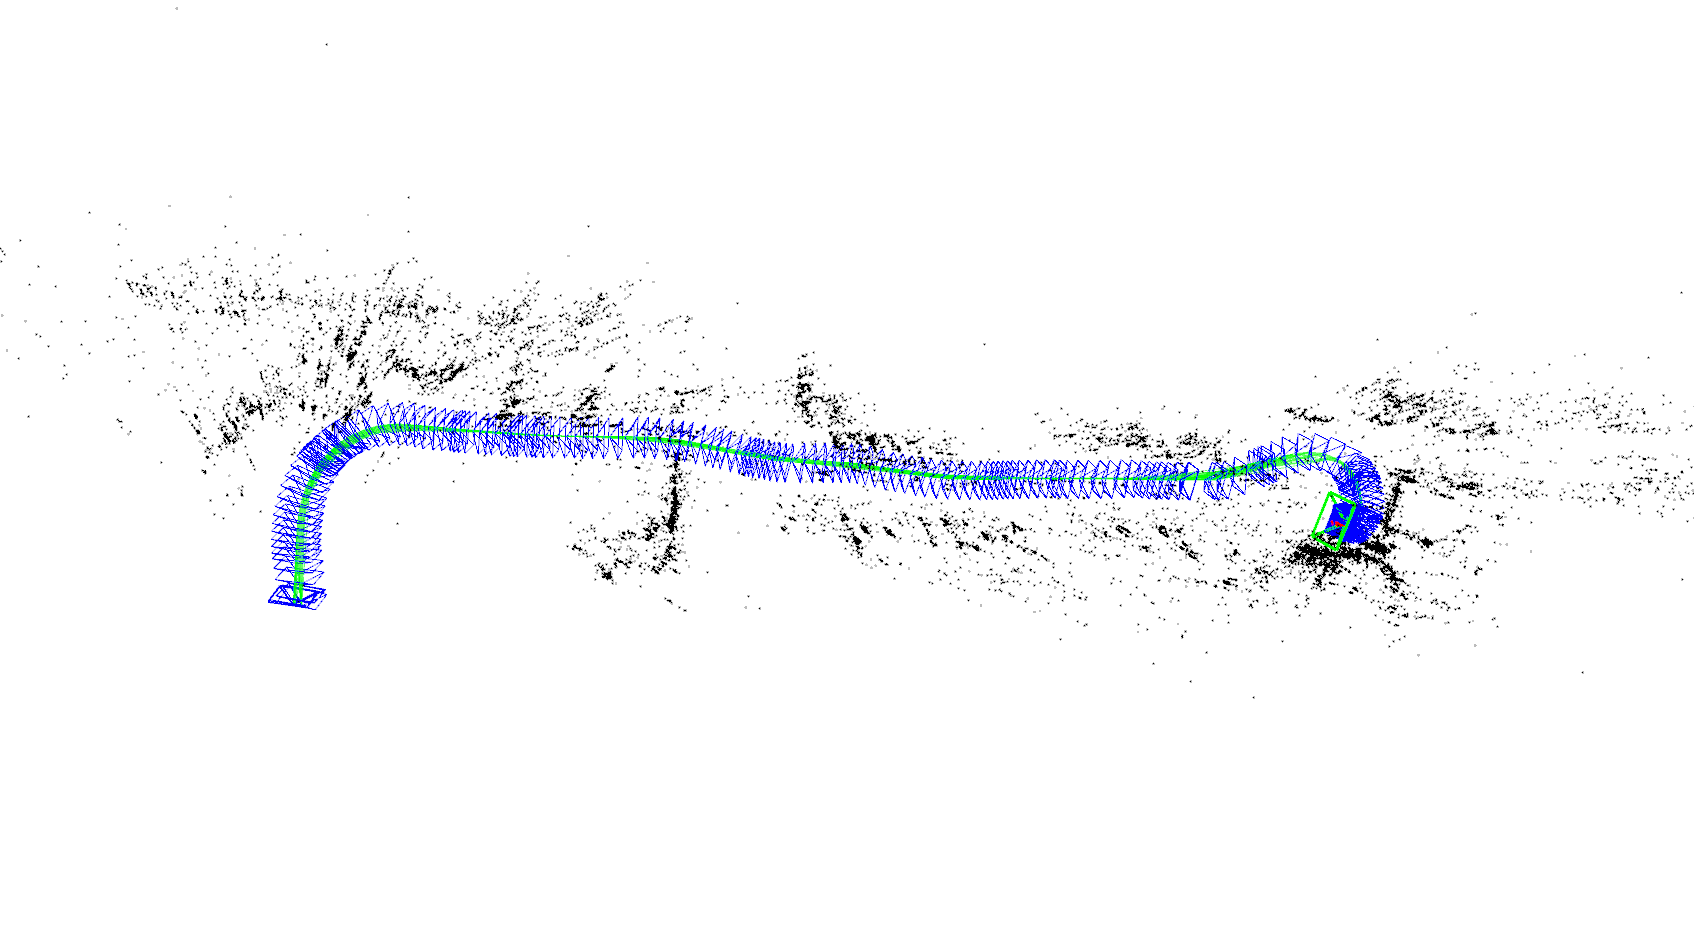
\includegraphics[width=.5\textwidth]{figures/demo2_ORB}%
	}
	\subfloat[]{%
		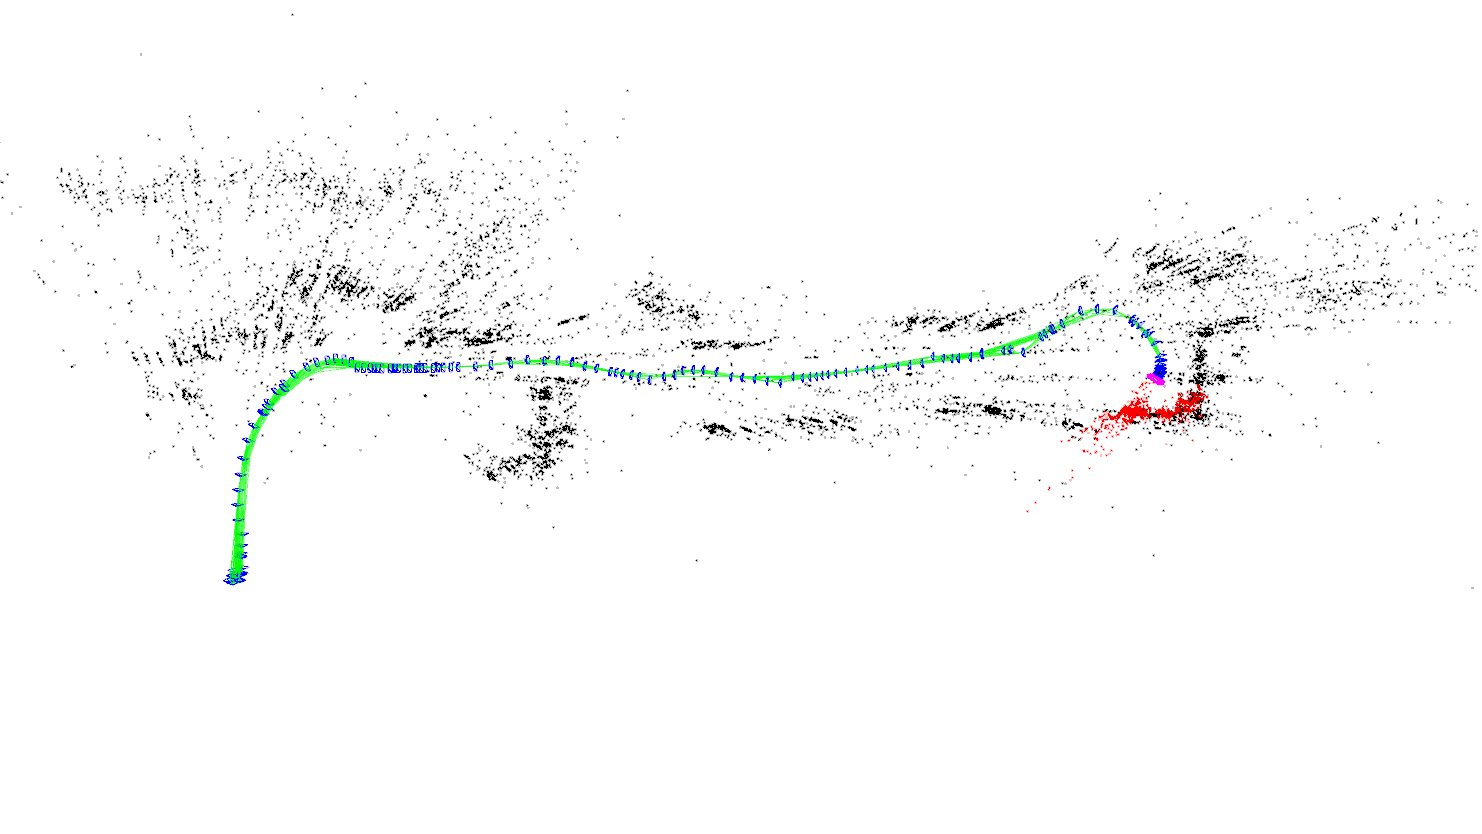
\includegraphics[width=.5\textwidth]{figures/demo2_VIORB}
	}
	\caption[Indoor experiment.]{\small 
		Indoor experiment. (a) Using ORB SLAM. (b) Using VIORB SLAM.}
	\label{fig:indoor-path-visualization}
	
\end{figure}

The trajectories of ORB SLAM and VIORB SLAM are compared in Figure~\ref{fig:indoor-experiment-trajectory}. VIORB SLAM's trajectory is closer to the real world trajectory, considering the distance calculated.

\begin{figure} [h]
	\centering
	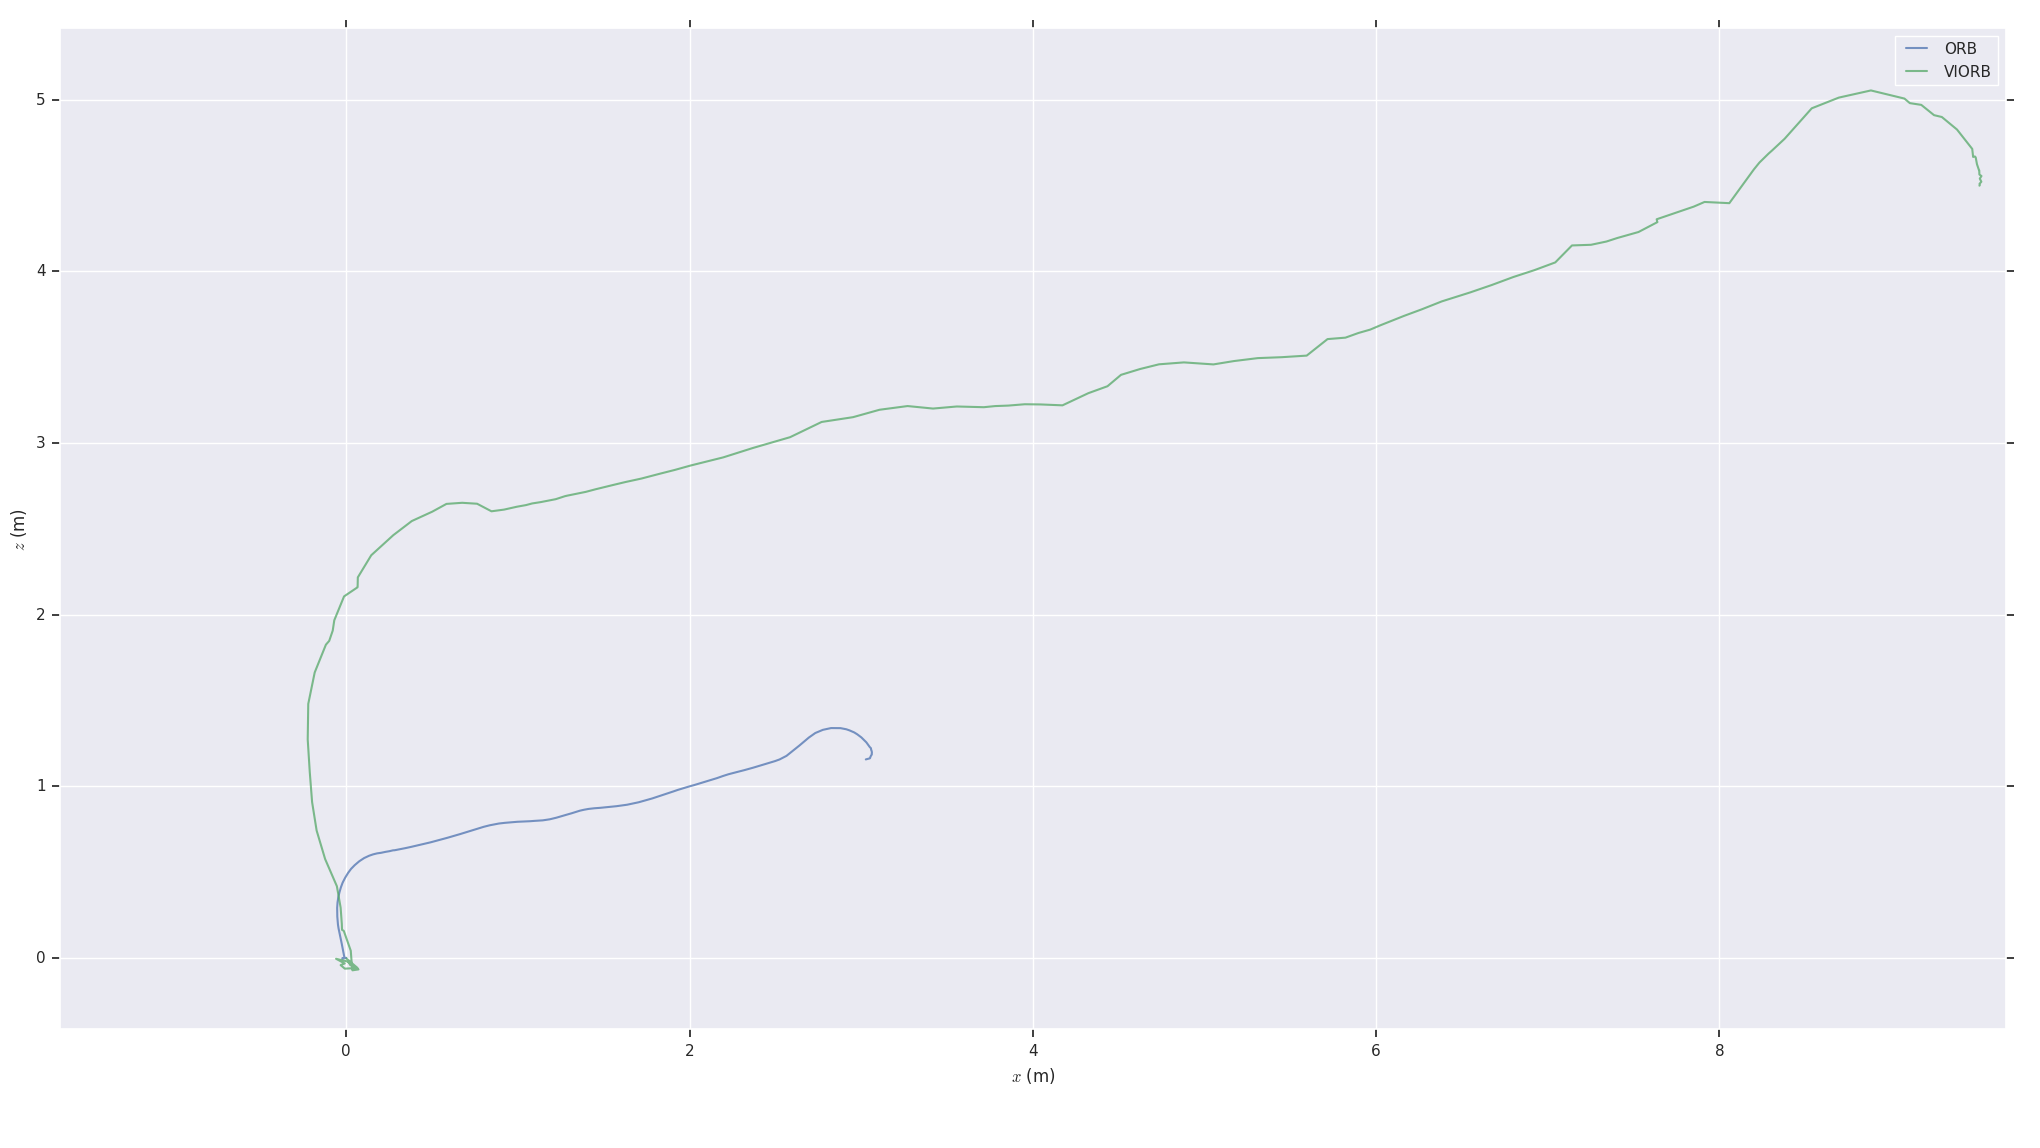
\includegraphics[width=5in]{figures/demo2_trajectory}
	\caption[Indoor experiment trajectory]{\small 
		Indoor experiment trajectory. }
	\label{fig:indoor-experiment-trajectory}
\end{figure}



\begin{table}[h]
	\caption[Comparision of ORB and VIORB SLAM in indoor environment.]{\small Comparision of ORB and VIORB SLAM in indoor environment.}
	\begin{tabular}{|c|c|c|c|c|c|}
		\hline 
		Algorithm & Total Time & IMU initialization time & Duration tracked & Poses & Path length \\ \hline \hline
		ORB & 170s & NA & 161.148s  & 249 & 3.920m  \\ \hline
		VIORB & 170s & 15s & 117.459s & 155 & 13.875m \\ \hline
	\end{tabular}
	\label{tab:indoor-comparision}
\end{table} 




\section {Outdoor Experiment}

The test rover was run in an outdoor environment for 173 seconds (Figure ~\ref{fig:outdoor-experiment-live}). As in the case of the indoor experiment, the number of ORB 
features to extract was kept at 2000 per frame. The keypoints, trajectory, and pointclouds generated by both algorithms are shown in Figure~\ref{fig:outdoor-path-visualization}. In this experiment, the IMU initialization time was increased to 30 seconds, from 10 seconds in the indoor experiment.

In the outdoor experiment, the rover faced more jerky movements than the 	indoor environment. VIORB SLAM re-localized for a couple of times. Then, it lost tracking when taking a left turn. ORB SLAM did not lose track for the entire test run.

\begin{figure}[h]
	\centering
	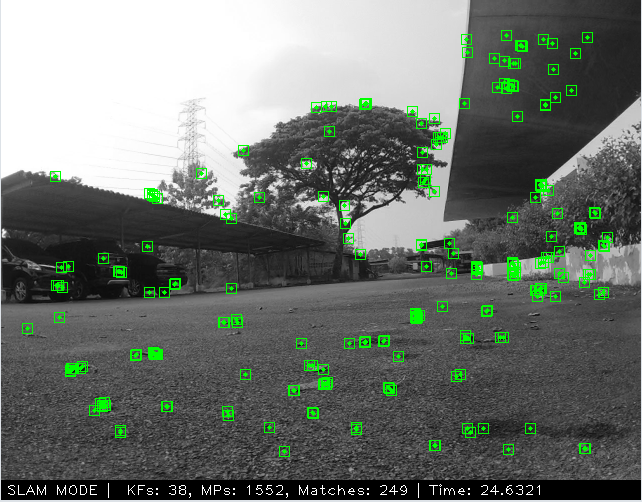
\includegraphics[width=5in]{figures/demo3_screen}
	\caption[Outdoor experiment environment]{\small 
		Outdoor experiment environment. }
	\label{fig:outdoor-experiment-live}
\end{figure}


\begin{figure}[h]
	
	\centering
	\subfloat[]{%
		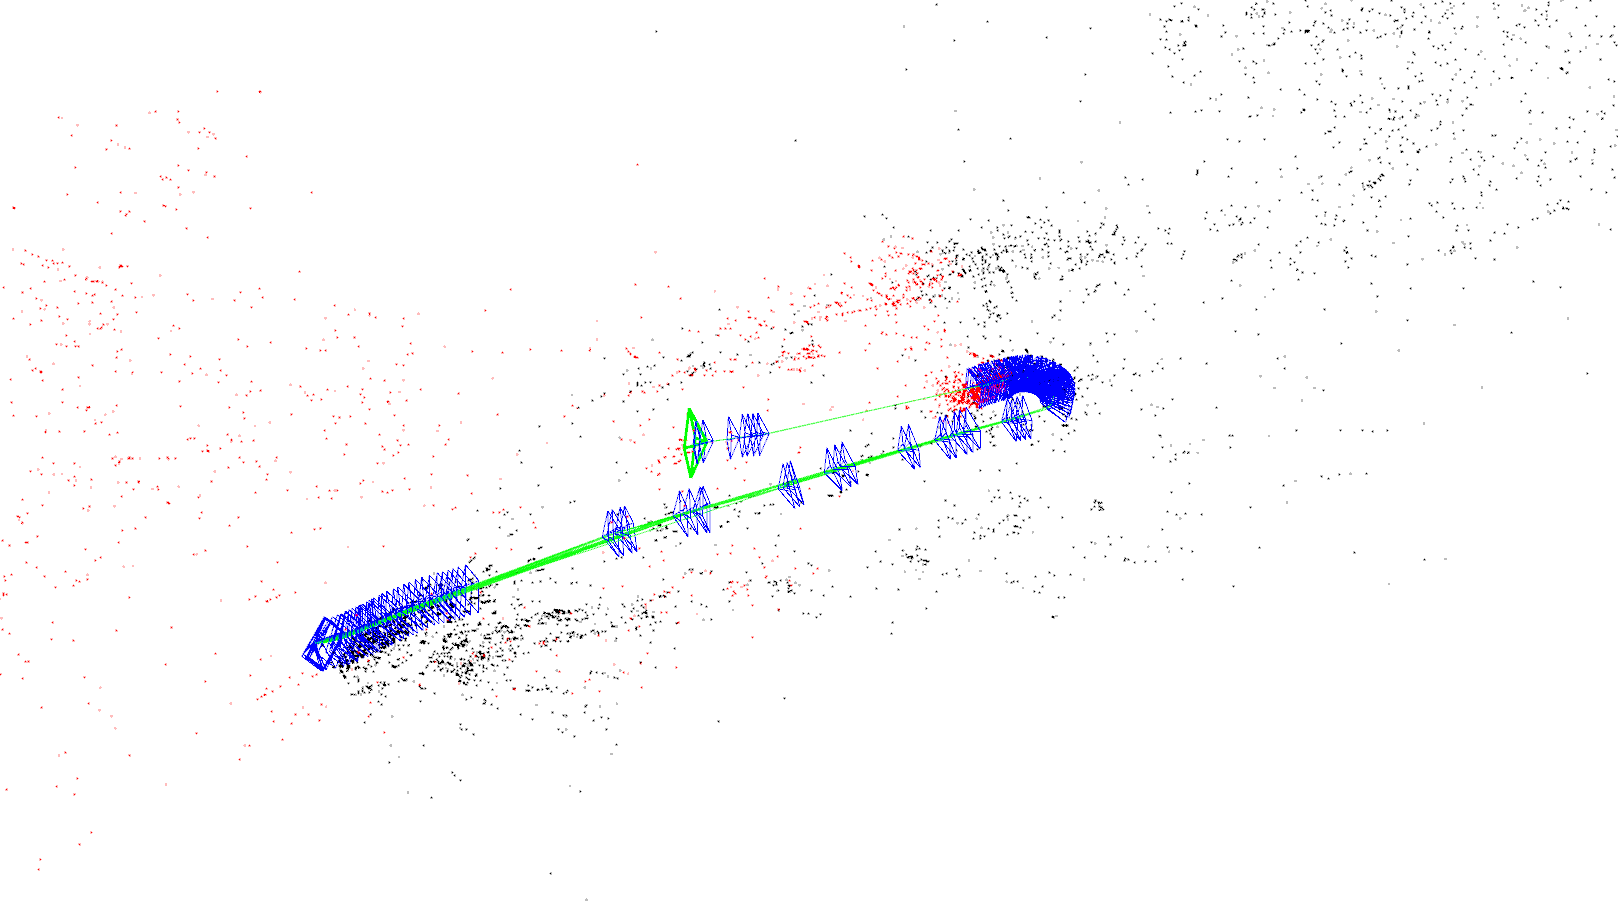
\includegraphics[width=.5\textwidth]{figures/demo3_ORB}%
	}
	\subfloat[]{%
		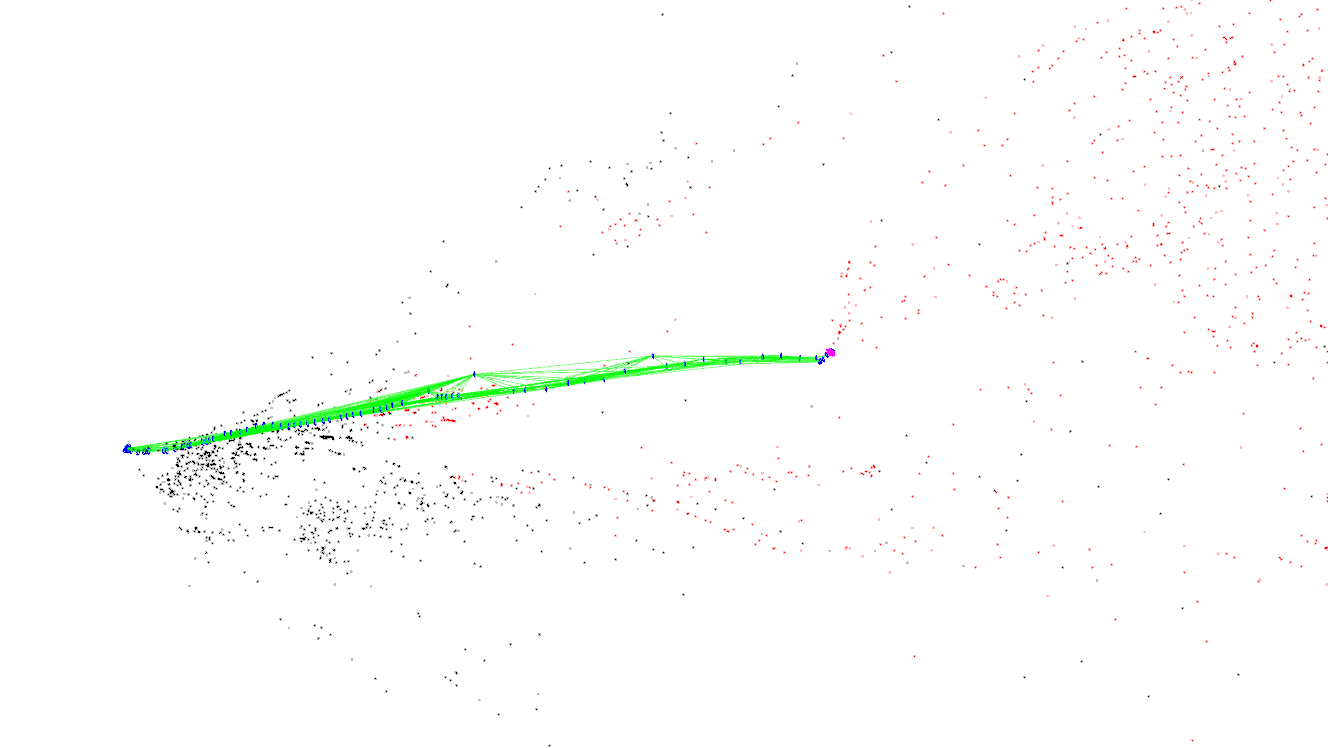
\includegraphics[width=.5\textwidth]{figures/demo3_VIORB}
	}
	\caption[Outdoor experiment.]{\small 
		Outdoor experiment. (a) Using ORB SLAM. (b) Using VIORB SLAM.}
	\label{fig:outdoor-path-visualization}
	
\end{figure}

The test rover was run on a straight line, a left u-turn followed by a straight line till halfway.
The trajectory of ORB SLAM and VIORB SLAM is compared in Figure~\ref{fig:outdoor-experiment-trajectory}. The trajectory calculated from GPS from the Pixhawk is shown in  Figure~\ref{fig:outdoor-experiment-gps-trajectory}. The GPS trajectory drifted a lot from the ground truth and is not reliable. But, the scale of the GPS trajectory and VIORB SLAM trajectory differs.

\begin{figure}[h]
	\centering
	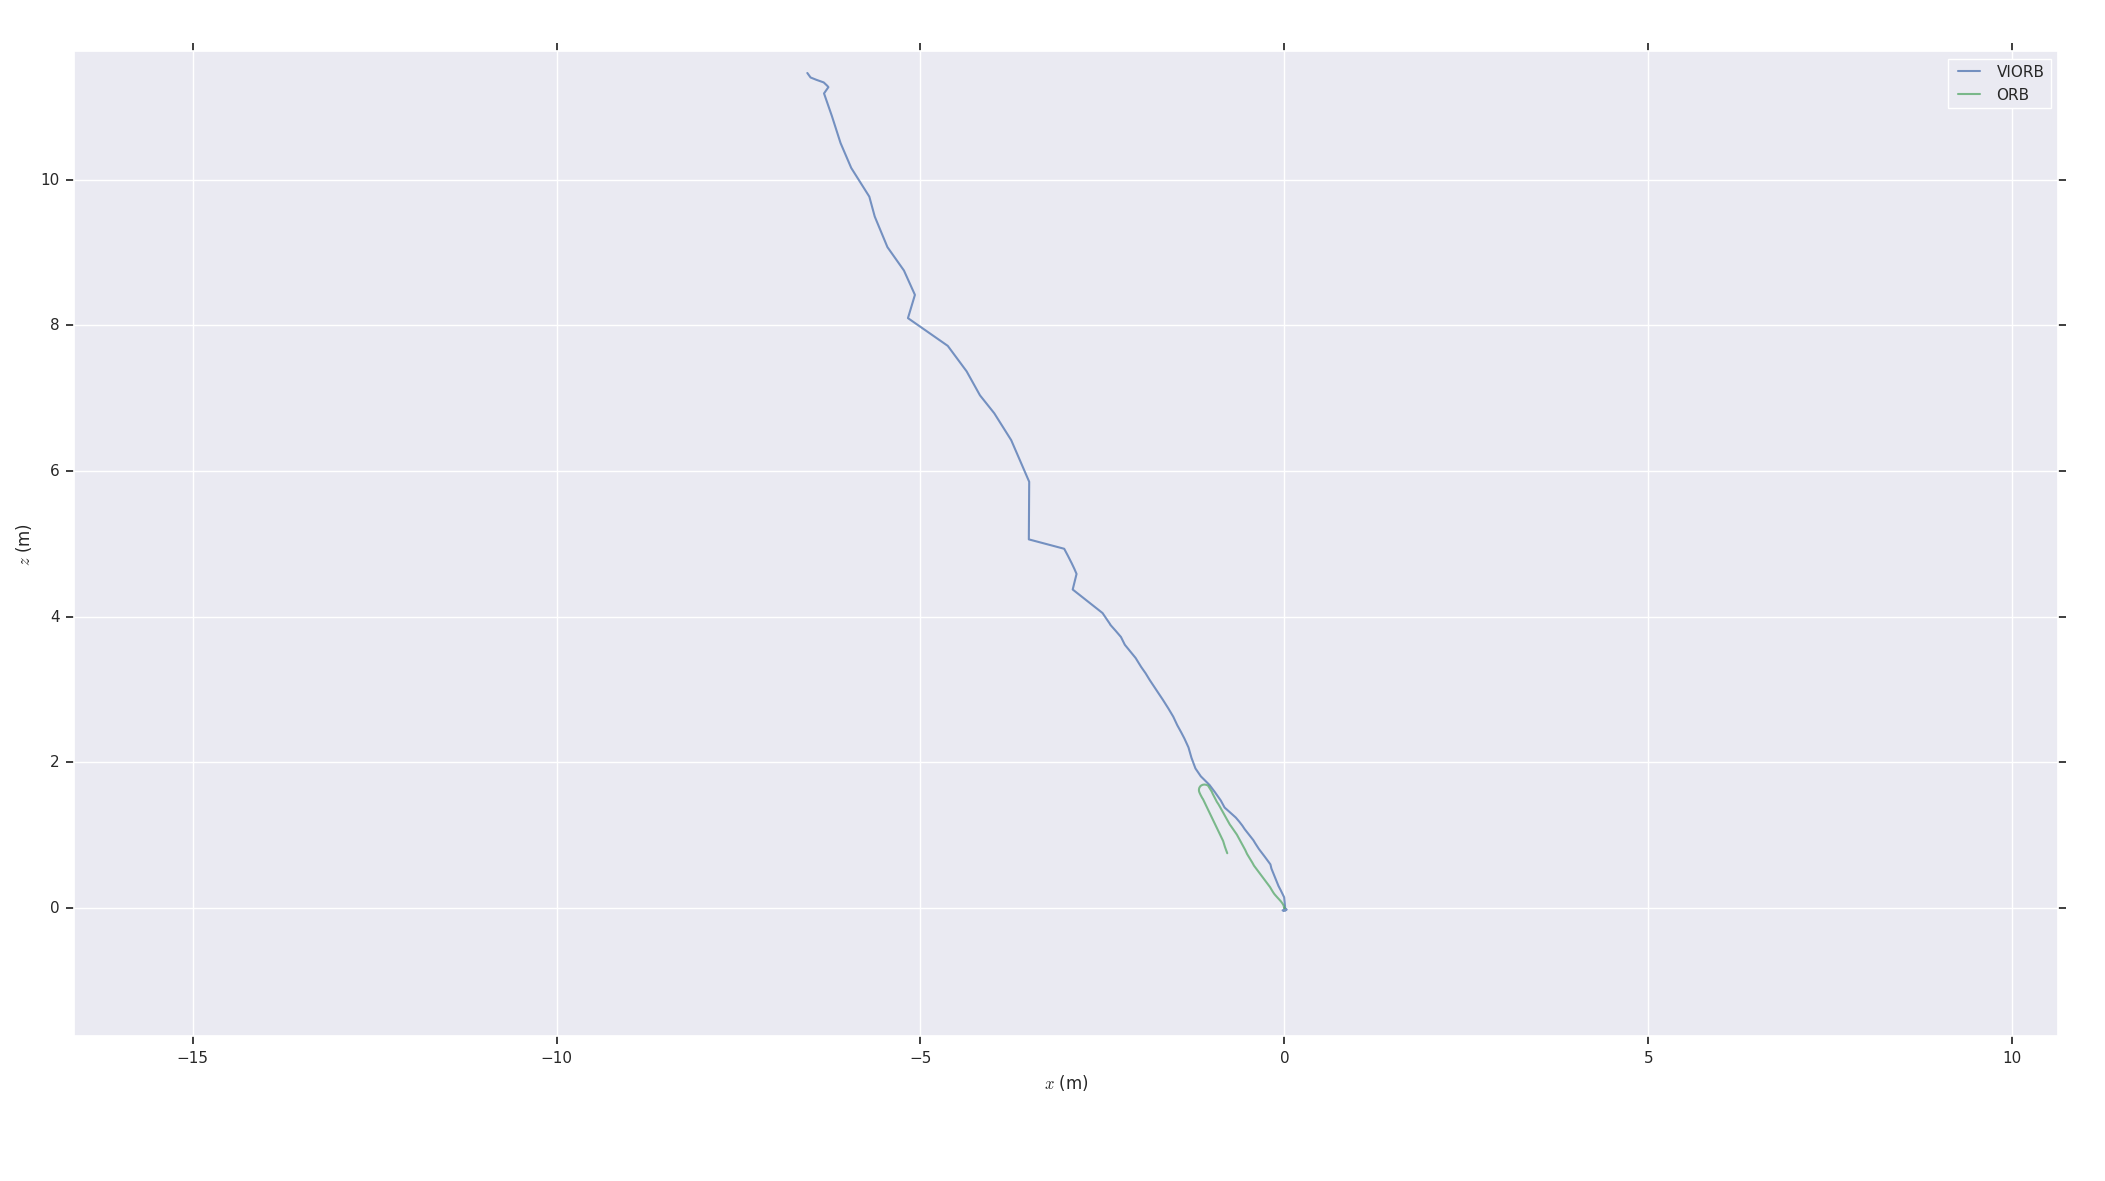
\includegraphics[width=5in]{figures/demo3_trajectory}
	\caption[Outdoor experiment trajectory]{\small 
		Outdoor experiment trajectory. }
	\label{fig:outdoor-experiment-trajectory}
\end{figure}

\begin{figure}[h]
	\centering
	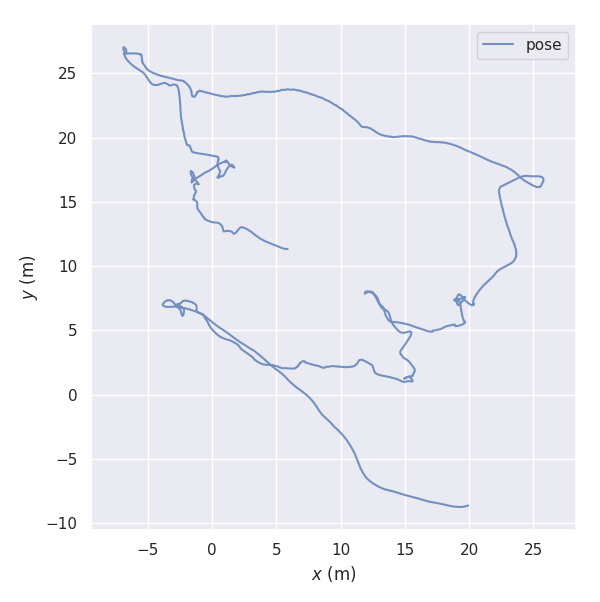
\includegraphics[width=5in]{figures/gps_trajectory}
	\caption[Outdoor experiment GPS trajectory]{\small 
		Outdoor experiment GPS trajectory. }
	\label{fig:outdoor-experiment-gps-trajectory}
\end{figure}


\begin{table}[h]
	\caption[Comparison of ORB and VIORB SLAM in outdoor environment.]{\small Comparison of ORB and VIORB SLAM in outdoor environment.}
	\begin{tabular}{|c|c|c|c|c|c|}
		\hline 
		Algorithm & Total Time & IMU initialization time & Duration tracked & Poses & Path length \\ \hline \hline
		ORB & 174s & NA & 160.637s  & 134 & 3.150m  \\ \hline
		VIORB & 174s & 30s & 96.871s & 85 & 14.427m \\ \hline
	\end{tabular}
	\label{tab:outdoor-comparision}
\end{table} 

\FloatBarrier

